


% Bounded identity
\begin{frame}{\tciii{} Signed distances}

\begin{columns}
\begin{column}{0.45\linewidth}
\begin{block}{Bounded identity function}
\begin{equation}
\alpha: \begin{cases}
& \text{ if } x \geq 1: \alpha(x) = 1\\ 
& \text{ if } x \leq -1: \alpha(x) = -1\\ 
& \text{ else: }  \alpha(x) = x
\end{cases}
\end{equation}
\end{block}
\end{column}

\begin{column}{0.45\linewidth}
\begin{figure}
\centering
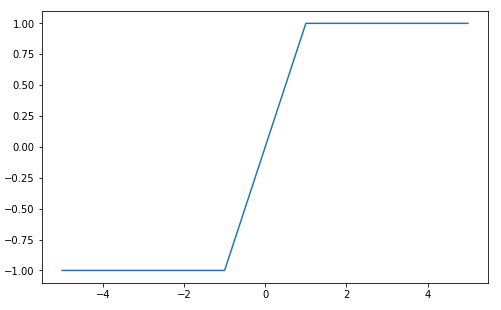
\includegraphics[width=.9\linewidth]{images/GENE/images/bounded.png}
\end{figure}
\end{column}
\end{columns}

\end{frame}


% Final functions
\begin{frame}{\tciii{} Distance functions}

\begin{columns}
\begin{column}{0.60\linewidth}
\begin{block}{pL2-GENE}
\begin{equation}
\alpha \left  ( \prod_{k=1}^D n_1^k - n_2^k \right ) \sqrt{\sum_{j=1}^D \left( n_1^j - n_2^j \right)^2 }
\end{equation}
\end{block}
\end{column}

\begin{column}{0.35\linewidth}
\begin{figure}
\centering
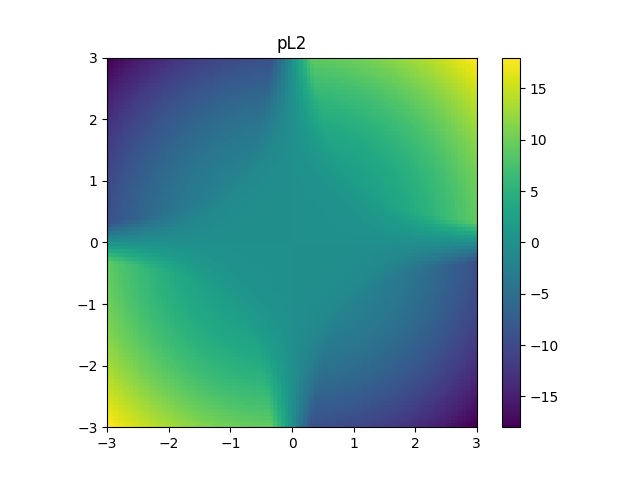
\includegraphics[width=\linewidth]{images/GENE/images/distance_pL2.png}
\end{figure}
\end{column}
\end{columns}

\begin{columns}
\begin{column}{0.60\linewidth}
\begin{block}{tag-GENE}
\begin{equation}
\sum_{j=2}^D \alpha(n_1^j - n_2^1) e^{-|n_1^j - n_2^1|}
\end{equation}
\end{block}
\end{column}

\begin{column}{0.35\linewidth}
\begin{figure}
\centering
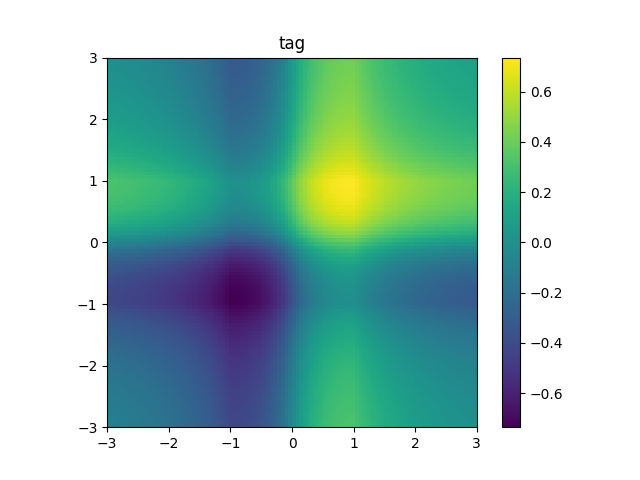
\includegraphics[width=\linewidth]{images/GENE/images/distance_tag.png}
\end{figure}
\end{column}
\end{columns}

\end{frame}


    